\documentclass[conference]{IEEEtran}
\IEEEoverridecommandlockouts

\usepackage{cite}
\usepackage[portuges,brazil,english]{babel}
\usepackage{amsmath,amssymb,amsfonts}
\usepackage{algorithmic}
\usepackage{graphicx}
\usepackage{textcomp}
\usepackage[latin1,utf8]{inputenc}
\usepackage{listings}
\usepackage{color}

% Commands to help in references
\newcommand{\rchap}[1]{Chapter~\ref{chap:#1}}
\newcommand{\rsec}[1]{Section~\ref{sec:#1}}
\newcommand{\rsecs}[2]{Sections~\ref{sec:#1} --~\ref{sec:#2}}
\newcommand{\rtab}[1]{Tabela~\ref{tab:#1}}
\newcommand{\rfig}[1]{Figura~\ref{fig:#1}}
\newcommand{\rfigs}[2]{Figures~\ref{fig:#1} --~\ref{fig:#2}}
\newcommand{\rfign}[3]{Figures~\ref{fig:#1}, \ref{fig:#2} \& \ref{fig:#3}}
\newcommand{\rlst}[1]{Listing~\ref{lst:#1}}
\newcommand{\rlsts}[2]{Listing~\ref{lst:#1}~--~\ref{lst:#2}}
\newcommand{\rlstn}[3]{Listings~\ref{lst:#1}{#2}~--~\ref{lst:#1}{#3}}
\newcommand{\req}[1]{Equation~\ref{eq:#1}}
\newcommand{\reqs}[2]{Equations~\ref{eq:#1} --~\ref{eq:#2}}
\newcommand{\ttt}[1]{{\texttt{#1}}}
\newcommand{\tbt}[1]{{\textbf{#1}}}
\newcommand{\tit}[1]{{\textit{#1}}}
\newcommand{\ts}{\textsuperscript}

\def\BibTeX{{\rm B\kern-.05em{\sc i\kern-.025em b}\kern-.08em
    T\kern-.1667em\lower.7ex\hbox{E}\kern-.125emX}}

\definecolor{codegreen}{rgb}{0,0.6,0}
\definecolor{codegray}{rgb}{0.5,0.5,0.5}
\definecolor{codepurple}{rgb}{0.58,0,0.82}
\definecolor{backcolour}{rgb}{0.95,0.95,0.92}
\definecolor{darkblue}{rgb}{0.0,0.0,0.6}

\lstdefinestyle{mystyle}{
  commentstyle=\foonotesize\color{codegreen},
  backgroundcolor=\color{backcolour},
  stringstyle=\color{codepurple},
  basicstyle=\footnotesize,
  breakatwhitespace=false,
  breaklines=true,
  captionpos=b,
  keepspaces=true,
  showspaces=false,
  showstringspaces=false,
  showtabs=false,
  tabsize=2
}

\lstset{
  classoffset=0,
  keywordstyle=\color{back},
  classoffset=1,
  morekeywords={use,hrw,module,increment,HARP,Catapult,synthesize},
  keywordstyle=\color{purple},
  classoffset=2,
  morekeywords={pragma,omp,parallel,target,map,data,device,for,},
  keywordstyle=\color{darkblue},
  frame=single,
  style=mystyle
}

\begin{document}

\title{Desmistificando o Cartola FC}

\author
{
  \IEEEauthorblockN{Ciro Ceissler}
  \IEEEauthorblockA{RA 108786\\ ciro.ceissler@gmail.com}
  \and
  \IEEEauthorblockN{Lucas de Souza e Silva}
  \IEEEauthorblockA{RA 140765\\ lucasonline1@gmail.com}
  \and
  \IEEEauthorblockN{Matheus Laborão Netto}
  \IEEEauthorblockA{RA 137019\\ mln.laborao@gmail.com}
  \and
  \IEEEauthorblockN{Ramon Nepomuceno}
  \IEEEauthorblockA{RA 192771\\ ramonn76@gmail.com}
}

\maketitle

\begin{abstract}

TODO(ciroceissler):

\end{abstract}

\section{Introdução}

O futebol é um esporte com diversos  fãs ao redor do mundo e com uma
imprevisibilidade muito grande, supreendendo os torcedores. Um exemplo
recente foi  a Copa  do Mundo de  2018 no qual  o campeão  do torneio
anterior não conseguiu passar nem da primeira fase, perdendo 2x0 para
Coreia do Sul apenas 57\ts{a}  colocada no ranking FIFA \cite{fifa}, e
a presença  Croácia na  final. Ainda nesta  Copa do  Mundo; diversos
bancos, incluindo  o \tit{Goldman Sachs}, utilizaram  este evento para
demonstrar a capacidade de  prever eventos complexos \cite{news}, eles
chegaram a  rodar milhões de  variações do torneio para  calcular a
probabilidade de cada time avançar na competição e mesmo assim não
obtiveram um resultado satisfatório.

Os fãs  de futebol  também participam  da "brincadeira"  através do
Cartola FC, um  "fantasy game" sobre este esporte. O  Cartola FC é um
jogo online fictício no qual você pode montar seu time com jogadores
reais da Série A do Campeonato  Brasileiro. No jogo é preciso montar
seu time, escolhendo  técnico, jogadores e o esquema  tático. Com as
moedas  do  jogo, inicialmente  C\$  100.00  cartoletas, é  possível
escalar  o seu  time, comprando  e vendendo  jogadores a  cada rodada,
importante  adicionar que  a  (des)valorização  do jogador  acontece
após cada  rodada e leva  em consideração a pontuação  do atleta,
além da  média dos  outros jogadores. A  escalação deve  ser feita
antes do  primeiro jogo da rodada  e a cada uma,  os jogadores recebem
pontuações  baseadas  em suas  ações  durante  as partidas,  e.g.,
gols feitos,  chutes defendidos,  bolas roubadas, faltas  cometidas ou
sofridas, cartões  recebidos, entre outras. As  ações dos jogadores
em campo são  chamadas de Scouts e são elas  que geram a pontuação
do time. Por fim, o Capitão tem sua pontuação duplicada e não pode
ser o  técnico. No Cartola FC  de 2017, o jogador  vencedor totalizou
2460.19 pontos ao final de todas as rodadas (média de 67.4 pontos por
rodada), competindo contra 4 milhões de times escalados.

O projeto propõe um modelo  preditivo para maximizar a pontuação do
Cartola FC, informando  a cada rodada do jogo  quais parâmetros devem
ser utilizados, ou seja, escolher  os jogadores/técnico a cada rodada
para o torneio de 2018.

\section{Trabalhos Relacionados}

TODO(ciroceissler): football
\cite{sugar2015predicting}
\cite{porter2018predictive}
\cite{lutz2015fantasy}
\cite{dolan2015machine}
\cite{becker2016analytical}

Em  \cite{viscondiaplicaccao},  um   sistema  de  previsão  aplicando
técnicas  de \tit{machine  learning}  foi proposto  para conseguir  a
melhor escalação do time a  em cada rodada, entretanto os resultados
obtidos não permitiria  vencer o torneio. Além  disso, este trabalho
fez uma análise  dos dados, explanando algumas  observações como: o
esquema  tático tem  uma  leve  variação, sendo  o  4-4-2 a  melhor
formação.

\cite{schmidt2017uso}

\cite{mota2018cartola}

\cite{gomide2018} \cite{git_cartola}

\section{Base de Dados}

A base de  dados \cite{git_cartola} contém as  informações sobre os
campeonatos  de 2014  a  2017 consolidadas  e  serão utilizadas  para
aprendizado do nosso  modelo, os dados sobre 2018  são adicionadas ao
término de cada rodada. No  repositório, cada campeonato é dividido
em cinco arquivos do formato \tit{csv} com as seguintes informações:
nome  dos  times,  posição  e time  dos  jogadores  (considera-se  o
técnico  um  jogador com  a  posição  de técnico),  resultado  das
partidas  do  campeonato,  lista  dos  scouts, e  a  tabela  final  da
pontuação dos times no campeonato.

\begin{table}[h]
\begin{center}
\caption[]{Tipos de Scouts}
\label{tab:model}
\begin{tabular}{| l | c | c | c | c | c | c | c | c | c | c |}
\hline
\multicolumn{2}{|c|}{Scouts de Ataque} & \multicolumn{2}{|c|}{Scouts de Defesa} \\
\hline
Gol                   &  8.0 pts & Jogo sem sofrer gols &  5.0 pts \\
Assistência           &  5.0 pts & Defesa de pênalti    &  7.0 pts \\
Finalização na trave  &  3.0 pts & Defesa difícil\ts{1} &  3.0 pts \\
Finalização defendida &  1.2 pts & Roubada de bola      &  1.5 pts \\
Finalização para fora &  0.8 pts & Gol contra           & -5.0 pts \\
Falta sofrida         &  0.5 pts & Cartão vermelho      & -5.0 pts \\
Pênalti perdido       & -4.0 pts & Cartão amarelo       & -2.0 pts \\
Impedimento           & -0.5 pts & Gol sofrido\ts{1}    & -2.0 pts \\
Passe errado          & -0.3 pts & Falta cometida       & -0.5 pts \\
\hline
\end{tabular}
\end{center}
\end{table}
% \ts{1}scots exclusivos de goleiro.

Abaixo, os  itens abaixo  complementam a \rtab{model}  com a  lista de
Scouts, também sendo atualizado a cada rodada:

\begin{itemize}

\item \textbf{atletas.nome:}                nome completo do jogador
\item \textbf{atletas.apelido:}             nome/apelido do jogador
\item \textbf{atletas.rodada\_id:}          número da rodada do Brasileirão
\item \textbf{atletas.clube\_id:}           abreviação do clube do jogador
\item \textbf{atletas.posicao\_id:}         posição do jogador
\item \textbf{atletas.clube.id.full\_name:} clube do jogador
\item \textbf{atletas.status\_id:}          status do jogador na rodada
\item \textbf{atletas.pontos\_num:}         pontuação dos scouts
\item \textbf{atletas.preco\_num:}          preço do jogador
\item \textbf{atletas.variacao\_num:}       variação do preço do jogador
\item \textbf{atletas.media\_num:}          média do jogador
\item \textbf{atletas.jogos\_num:}          quantidade de jogos disputados
\item \textbf{atletas.scout:}               quantidade de scouts obtidos

\end{itemize}

\section{Tratamento dos Dados}

Antes  de realizar  o treinamento,  uma análise  dos dados  foi feita
de  maneira  preliminar para  identificar  quais  melhorias podem  ser
realizadas, além  de eliminar inconsistências no  arquivo, utilizado
como entrada para o treinamento do modelo.

\subsection{Limpeza}

A primeira  etapa realizada  para implementar  o modelo  de predição
foi  analisar os  dados fornecidos  pela  API do  cartola, fazendo  as
limpezas necessárias para criar amostras corretas e relevantes para o
preditor. Os  dados devem  continuar consistente  após a  limpeza dos
dados, ou  seja, nenhuma  coluna poderá  ser adicionada,  alterada ou
removida. Após uma análise prévia dos dados, alguns problemas foram
detectados nas informações dos jogadores:

\begin{itemize}
  \item todos os scouts com valor NaN (\tit{not a number}).
  \item coluna 'ClubeID' com valor NaN.
  \item coluna 'Status' com valor NaN.
  \item pontuação não equivalente a soma ponderada dos scouts.
\end{itemize}

A coluna  'atletas.clube\_id' tem campos repetidos  e divergentes: por
exemplo, todos os Atléticos (MG, PR, e GO) são ATL. Além disso, há
jogadores  com  siglas diferentes  das  equipes  que eles  jogam  (por
exemplo,  Maicosuel [id:  37851]).  A coluna  'athletes.atletas.scout'
não é informativa. Os scouts de 2015 dos jogadores são cumulativos,
ou seja,  os scouts dos  jogadores vão  sendo somados a  cada rodada.
Entretanto, a pontuação não é. Isso também causa o repetimento de
dados.

As linhas que possuem as inconsistências citadas acima são removidas
ou  atualizadas. Além  destas  modificações,  outras remoções  de
dados  irrelevantes são  realizadas, por  exemplo jogadores  que não
participaram de  nenhuma rodada, técnicos e  jogadores sem posição,
jogadores sem nome, entre outros.

\subsection{Atualização dos scouts cumulativos de 2015}

Como  dito  anteriomente, os  dados  sobre  os  scouts de  2015  foram
disponibilizados  de maneira  cumulativa pela  fornecidos pela  API do
cartola, ou seja, os scouts de  uma rodada são adicionados aos scouts
anteriores a cada nova rodada  que um jogador participa. Portanto, foi
necessário tirar essa acumulação para  cada jogador, de maneira que
a representação dos dados ficasse coerente.

Para isso, dada  uma rodada específica, os scouts de  um jogador são
subtraídos  do máximo  dos scouts  de todas  as rodadas  anteriores.
Repare que assim  há chance do scout 'Jogo Sem  Sofrer Gols (SG)' ser
negativo se o jogador não sofrer  gols na rodada anterior e sofrer na
rodada atual. Quando isso acontece, esse scout é atualizado.

\subsection{Verificação da pontuação com os scouts}

Por inconsistência  na base de  dados fornecida pela API  do cartola,
alguns  jogadores possuiam  pontuações que  não condiziam  com seus
scouts. Para esses casos, o jogador  é removido da base de dados para
evitar qualquer tipo de ruído. Ao final, mais de 4000 jogadores foram
removidos.

\subsection{Remoção das linhas duplicadas}

A última operação realizada para limpar  a base de dados foi apagar
as  linhas repetidas.  A existência  de linhas  repetidas deve-se  ao
fato  de que  a partir  da primeira  participação de  um jogador  no
campeonato, ele  aparece em todas  as rodadas subsequentes,  mesmo que
não tenha jogado.  As entradas redundantes não  são necessárias ao
modelo, por isso foram removidas.

\subsection{Criação das Amostras}

Continuando  a implementação  após a  limpeza da  base de  dados, o
próximo passo  foi transformar os  dados para tornar  utilizáveis na
criação dos modelos. Desta forma, duas operações são realizadas e
descritadas abaixo:

\begin{itemize}

\item  \textbf{Selecionar somente  as colunas  de interesse:}  colunas
como  'atletas.nome', 'atletas.foto',  etc não  são relevantes  para
criação  do  modelo.  No  entanto,   colunas  como  o  'AtletaID'  e
'atletas.apelido',  mesmo  que  não utilizadas  para  treinamento  do
modelo, são importante para avaliar  o resultado e, portanto, também
serão consideradas.

\item \textbf{Converter todos os  dados categóricos para numéricos:}
as   colunas  'Posicao',   'ClubeID',  'opponent'   e  'casa'   serão
convertidas para número.

\end{itemize}

\section{Treinamento}

O problema se encaixa na categoria de esportes, ou seja, na , que é comumente
resolvido através de um regressão linear para prever

Nesse método, todas as  combinações possíveis entre os parâmetros

As variações de soluções da regressão

Os    dados    foram    normalizados    utilizando    a    estratégia
\tit{MinMaxScaler}, que normaliza cada atributo no intervalo [0-1].

\subsection{Redes Neurais}

O  primeiro modelo  preditor consiste  numa rede  neural artificial  e
diferentes configurações para avaliar o desempenho delas. Em resumo,
o  seu funcionamento  acaba sendo  bem simples,  o modelo  recebe como
entrada os  dados de uma determinada  rodada e faz uma  predição das
pontuações dos jogadores para a próxima rodada.

Para   estimar  a   melhor  arquitetura   para  rede,   bem  como   os
hiperparâmetros,  foi  utilizada a  estratégia  \textit{GridSearch}.
Nesse método, todas as  combinações possíveis entre os parâmetros
são  testados usando  uma validação  cruzada com  5 \tit{folds}.  A
combinação de parâmetros que for  melhor na média dos \tit{folds},
é considerada a  melhor. As seguintes combinações  de redes neurais
foram utilizadas  com a  numeração de cada  item corresponde  ao seu
\ttt{id}:

\begin{enumerate}

\item quatros camadas escondidas cada uma com 50 neurônios.

\item três camadas escondidas sendo  os número de neurônios de cada
uma delas é, respectivamente, 50, 100, 50.

\item quatro camadas escondidas sendo os número de neurônios de cada
uma delas é, respectivamente, 50, 100, 100, 50.

\item apenas uma camada escondida com 128 neurônios.

\item duas camadas escondidas cada uma com 128 neurônios.

\item três camadas escondidas cada uma com 128 neurônios.

\end{enumerate}

% Optou-se  também por  normalizar  os dados  utilizando a  estratégia
% \tit{MinMaxScaler}, que normaliza cada  atributo no intervalo [0-1], e
% utilizar  o  método  de  otimização \tit{adam}.  \tit{Adam}  é  um
% algoritmo de  otimização que pode  ser usado em vez  do procedimento
% clássico de descida de gradiente estocástico para atualizar os pesos
% da rede de forma iterativa com base nos dados de treinamento.

Uma  vez que  trata-se de  um problema  de regressão,  a função  de
ativação da saída  escolhida para a rede foi a  função linear e a
rede  será  treinada visando  minimizar  a  Root Mean  Squared  Error
(RMSE).

A  \rtab{experiments}  mostra  o resultado  da  estratégia  comentada
acima  para diferentes  configurações de  redes neurais,  variando a
quantidade de  camadas escondidas  e seus neurônios.  Os \tit{scores}
negativos obtidos indicam  que os modelos avaliados  tem um desempenho
muito  ruim,  a documentação  do  \ttt{scikit-learn}  informa que  o
melhor score seria 1.

\begin{table}[h]
\caption[]{Experimentos das Redes Neurais}
\label{tab:experiments}
\begin{tabular}{l|llllll}
\tbf{id} & \tbf{fold 1} & \tbf{fold 2} & \tbf{fold 3} & \tbf{fold 4} & \tbf{fold 5} & \multicolumn{1}{c}{\tbf{média}} \\
\hline
1 & -19.514 & -22.250 & -19.641 & -19.224 & -17.298 & -18.879 \\
2 & -22.382 & -19.712 & -19.404 & -19.025 & -17.154 & -18.601 \\
3 & -17.114 & -19.669 & -22.350 & -19.490 & -19.038 & -18.585 \\
4 & -19.791 & -19.503 & -22.334 & -19.013 & -17.163 & -18.562 \\
5 & -22.282 & -19.824 & -20.116 & -17.211 & -19.424 & -18.592 \\
6 & -19.796 & -17.251 & -19.702 & -19.019 & -22.412 & -18.843
\end{tabular}
\end{table}

A melhor arquitetura  foi a que utiliza apenas uma  camada escondida e
128 neurônios, sendo  a média do seu \tit{score} igual  a -18.562. O
resultado mostra  que novas arquiteturas precisam  ser exploradas para
conseguir  melhorar  este resultado,  uma  vez  que as  redes  neurais
testadas  tem comportamento  muito similar  entre elas.  O \tit{score}
para  o  conjunto  de  validação foi  de  -18.962  pelos  resultados
analisados anteriormente esse baixo desempenho já era esperado.

\subsection{Regressão Linear: Random Forest}

\subsection{Regressão Linear: Ridge}

A regressão linear de Ridge, chamada também regularização de Tikhonov,
é um método para solucionar problemas

\begin{equation}
  J(w)=\lambda\norm{w}^2 + \sum_i (w^T x_i - y_i)^2.
\end{equation}

\subsection{Regressão Linear: Bayesian Ridge}

% TODO(ciroceissler: parameters
%
% alpha_1  = [1e-7, 1e-6, 1e-5]
% alpha_2  = [1e-7, 1e-6, 1e-5]
% lambda_1 = [1e-7, 1e-6, 1e-5]
% lambda_2 = [1e-7, 1e-6, 1e-5]

\subsection{Regressão Linear: ElasticNet}

\cite{zou2005regularization}

\subsection{Regressão Linear: Gradient Boosting}

\subsection{Regressão Linear: SVR (Support Vector Regression)}

\section{Resultados}

Os modelos descritos  na seção anterior foram todos  validados com o
conjunto de treinamento,  após tratamento dos dados,  e compreende os
anos de  2014 até 2016.  Os dados do  campeonato de 2017  foi tratado
como o  conjunto de validação,  ou seja, utiliza-se para  comparar a
performance do modelo e definir qual será escolhido para a fase final
dos experimentos.

\subsection{Conjunto de Validação}

O  conjunto  de validação  contempla  a  temporada  2017 na  qual  o
vencedor totalizou  2460.19 pontos  com uma média  de 67.4  pontos. A
\rtab{experiments_validation}  contém as  métricas avalidas  em cada
modelo com  os melhores  parâmetros explorados.  O modelo  com melhor
desempenho  e menor  variação foi  a regressão  linear de  Bayesian
Ridge,  com uma  média  de 55.79  pontos,  levando em  consideração
apenas da  rodada 6  até 38.  Outro fator que  pode ter  impactado no
resultado  abaixo do  campeão  foi  a não  inclusão  do técnico  e
capitão.

\begin{table}[h]
\caption[]{Experimentos de Validação}
\label{tab:experiments_validation}
\begin{tabular}{l|ccccc}

Modelo & Score & Média & \sigma & Total de Pontos \\

\hline

Redes Neurais     & -19.25 & 49.37 & 15.25 & 1629.20  \\
Random Forest     &  -0.03 & 35.75 & 16.72 & 1179.90  \\
Bayesian Ridge    &   0.01 & 55.79 & 14.59 & 1841.29  \\
Ridge             & NaN    & 52.59 & 18.27 & 1735.69  \\
ElasticNet        & NaN    & 55.35 & 15.71 & 1826.70  \\
Gradient Boosting &  -0.01 & 39.15 & 19.14 & 1291.80  \\
SVR               &  -0.17 & 30.88 & 17.75 & 1019.00

\end{tabular}
\end{table}

A \rfig{bar_round}  complementa os resultados da  tabela, mostrando os
pontos  obtidos por  cada modelo  para  cada rodada  comparando com  o
campeão  da temporada.  O campeão,  com  a cor  azul, acaba  ganhado
praticamente todas as rodadas quando  comparado com os outros modelos,
ocorrendo apenas alguns  casos esporádicos de resultado  ruim como na
rodada 10 e  30. O modelo do Bayesian Ridge  mantém um equilíbrio ao
longo  das rodadas  sempre  próximo  dos outros  modelos  e quando  o
resultado obtido a perda é moderada.

\subsection{Conjunto de Teste}

O  conjunto  de teste  compreende  o  Campeonato Brasileiro  de  2018,
finalizado no dia 02 de dezembro, no qual houve a participação de 20
times e um total de 38  rodadas. O campeão dessa temporada do Cartola
FC foi  Mateus Gomes Soares  com o  time Flajuveteus FC,  acumulando o
total de 3288.15 pontos com uma média de 86.53 pontos por rodada.

TODO(ciroceissler): nossa media pontuação.

TODO(ciroceissler): comparar rodada a rodada.

\section{Conclusão}

Neste projeto, criamos um modelo para prever a melhor escalação para
cada rodada do \tit{fantasy game}  Cartola FC. Diversas técnicas para
modelar o  problema foram analisadas,  testando a eficiência  de cada
modelo. O teste  utilizou a temporada de 2014 a  2016 como conjunto de
treinamento e a temporada de  2017 como validação. Ao final, optamos
por utilizar o Bayesian Ridge por causa do melhor desempenho comparado
aos  demais modelos  e  testamos  com a  última  temporada 2018,  que
finalizou no dia 02 de novembro.

TODO(ciroceissler): o resultado final foi.

TODO(ciroceissler): analise superficial dos dados.

\begin{figure*}[H]
  \vspace{-0.5cm}
  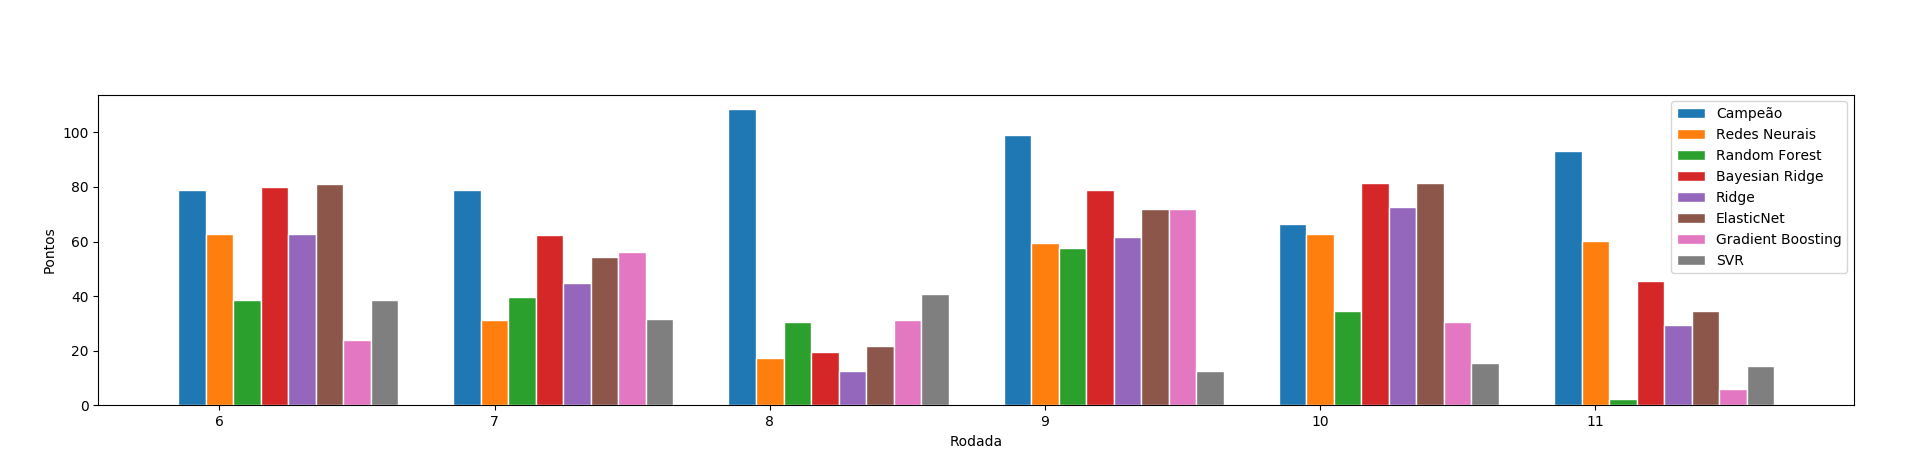
\includegraphics[trim={0 1.3cm 0 0}, clip, width=\textwidth]{images/bar_1.png}
  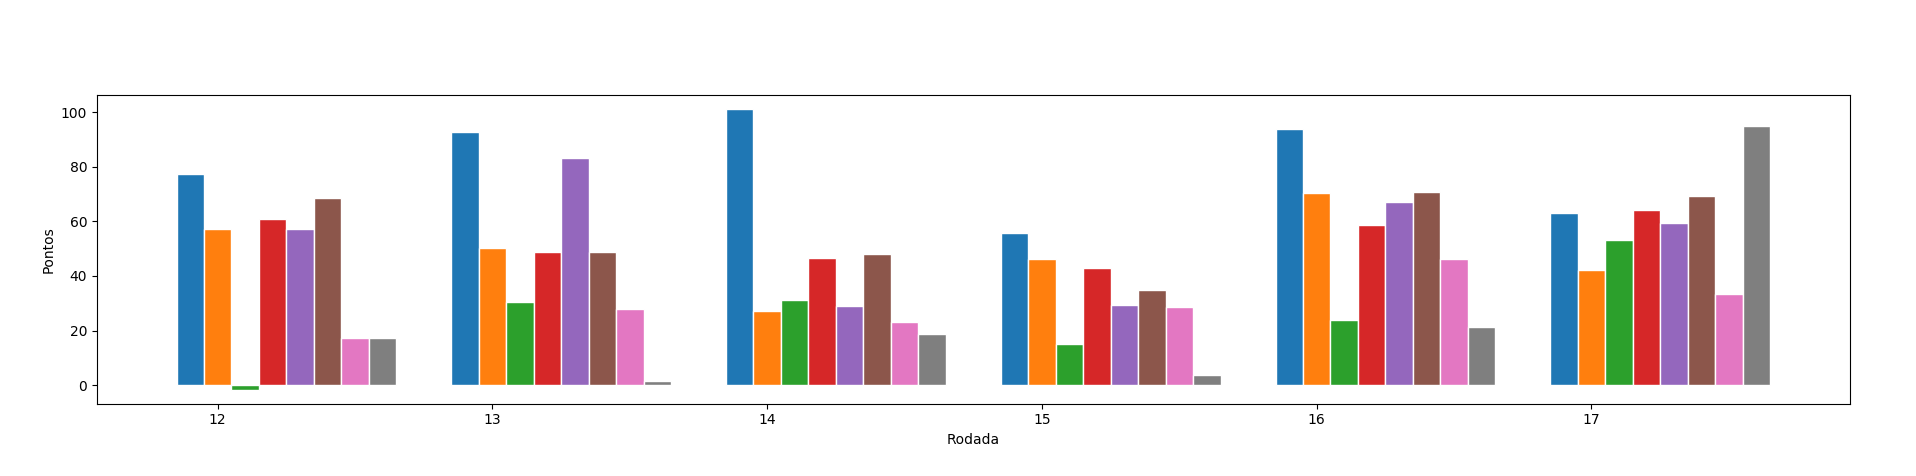
\includegraphics[trim={0 1.3cm 0 0}, clip, width=\textwidth]{images/bar_2.png}
  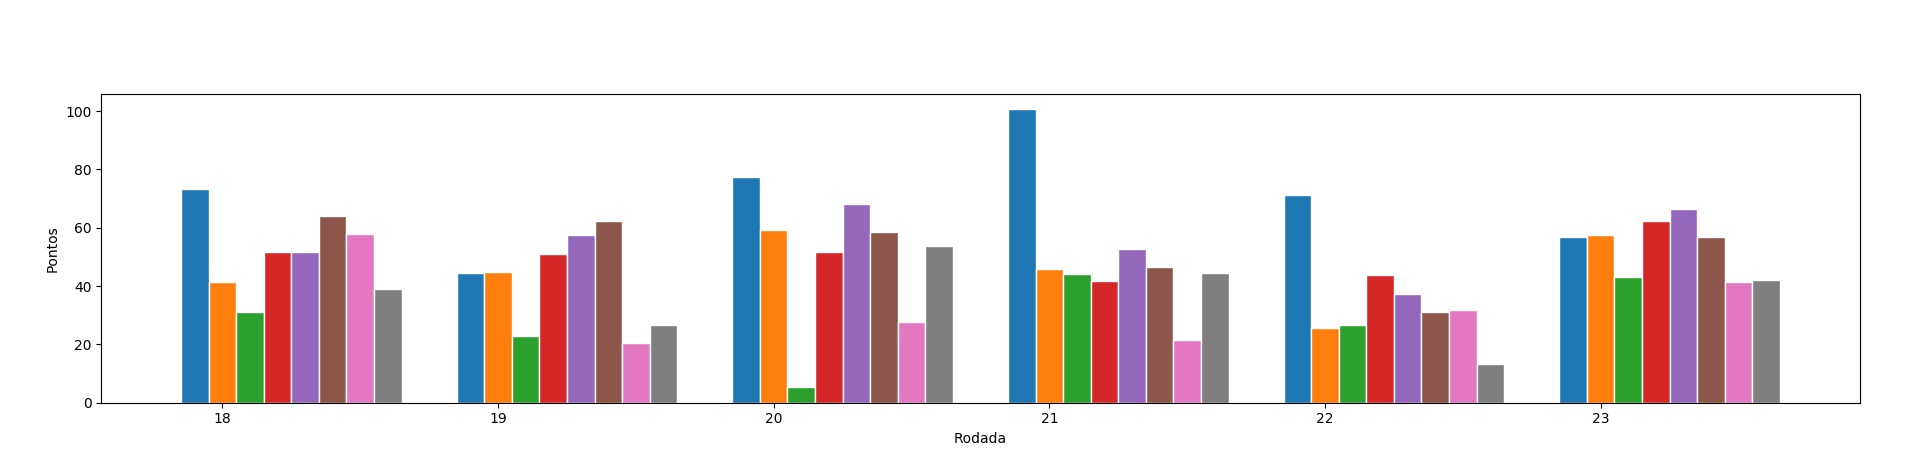
\includegraphics[trim={0 1.3cm 0 0}, clip, width=\textwidth]{images/bar_3.png}
  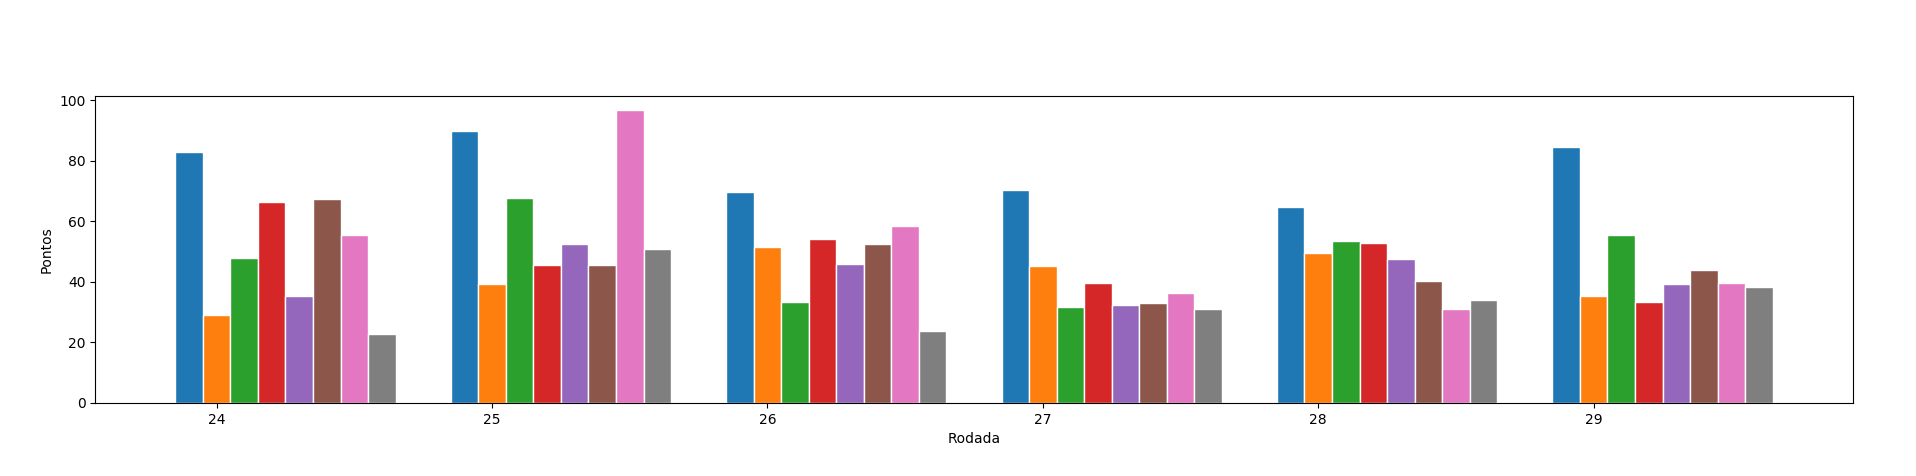
\includegraphics[trim={0 1.3cm 0 0}, clip, width=\textwidth]{images/bar_4.png}
  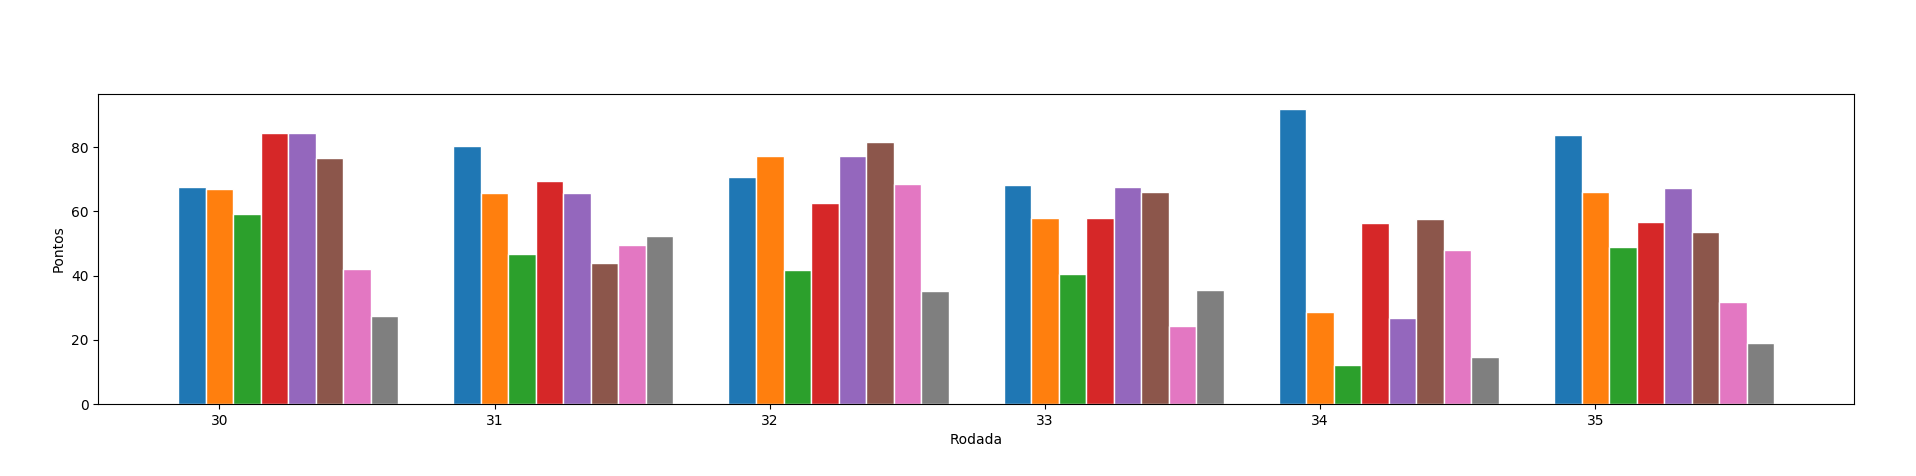
\includegraphics[trim={0 1.3cm 0 0}, clip, width=\textwidth]{images/bar_5.png}
  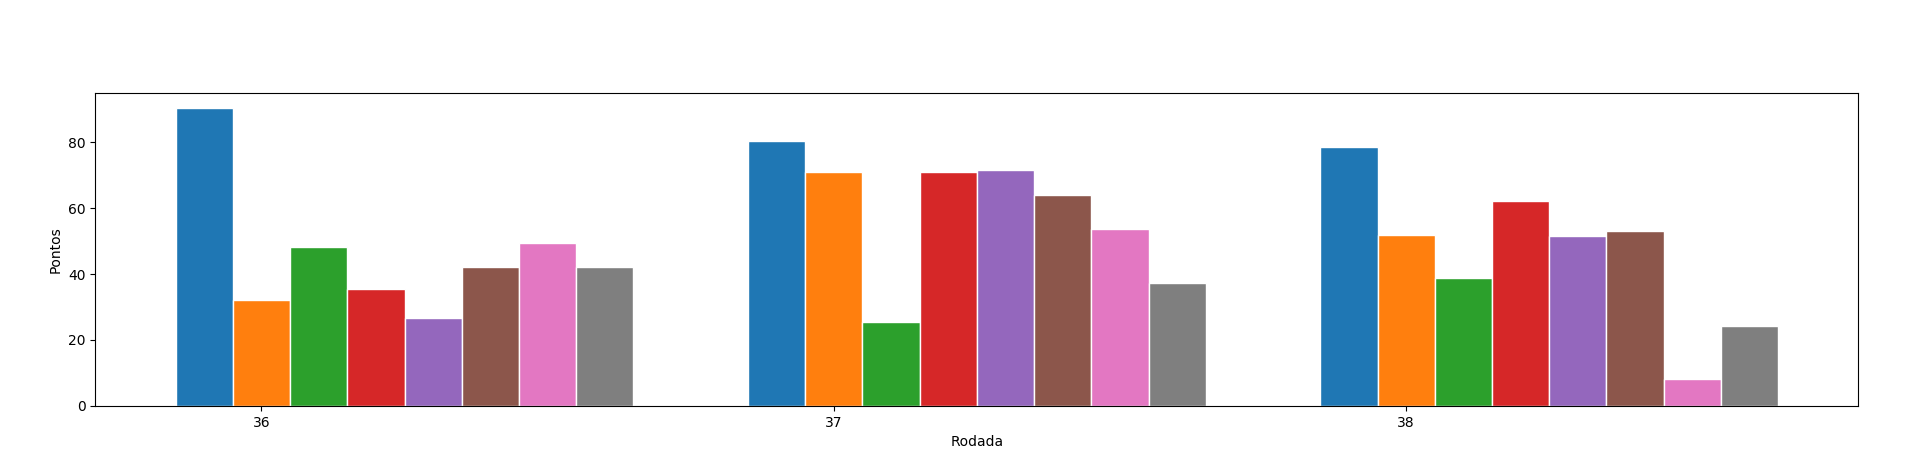
\includegraphics[width=\textwidth]{images/bar_6.png}
  \caption{Experimentos Temporada 2017 - Pontuação por Rodada para cada Modelo}
  \label{fig:bar_round}
\end{figure*}

\pagebreak

\nocite{*}
\bibliographystyle{IEEEtran}
\bibliography{report}

\end{thebibliography}

\end{document}
